% Options for packages loaded elsewhere
% Options for packages loaded elsewhere
\PassOptionsToPackage{unicode}{hyperref}
\PassOptionsToPackage{hyphens}{url}
\PassOptionsToPackage{dvipsnames,svgnames,x11names}{xcolor}
%
\documentclass[
  letterpaper,
  DIV=11,
  numbers=noendperiod]{scrartcl}
\usepackage{xcolor}
\usepackage{amsmath,amssymb}
\setcounter{secnumdepth}{-\maxdimen} % remove section numbering
\usepackage{iftex}
\ifPDFTeX
  \usepackage[T1]{fontenc}
  \usepackage[utf8]{inputenc}
  \usepackage{textcomp} % provide euro and other symbols
\else % if luatex or xetex
  \usepackage{unicode-math} % this also loads fontspec
  \defaultfontfeatures{Scale=MatchLowercase}
  \defaultfontfeatures[\rmfamily]{Ligatures=TeX,Scale=1}
\fi
\usepackage{lmodern}
\ifPDFTeX\else
  % xetex/luatex font selection
\fi
% Use upquote if available, for straight quotes in verbatim environments
\IfFileExists{upquote.sty}{\usepackage{upquote}}{}
\IfFileExists{microtype.sty}{% use microtype if available
  \usepackage[]{microtype}
  \UseMicrotypeSet[protrusion]{basicmath} % disable protrusion for tt fonts
}{}
\makeatletter
\@ifundefined{KOMAClassName}{% if non-KOMA class
  \IfFileExists{parskip.sty}{%
    \usepackage{parskip}
  }{% else
    \setlength{\parindent}{0pt}
    \setlength{\parskip}{6pt plus 2pt minus 1pt}}
}{% if KOMA class
  \KOMAoptions{parskip=half}}
\makeatother
% Make \paragraph and \subparagraph free-standing
\makeatletter
\ifx\paragraph\undefined\else
  \let\oldparagraph\paragraph
  \renewcommand{\paragraph}{
    \@ifstar
      \xxxParagraphStar
      \xxxParagraphNoStar
  }
  \newcommand{\xxxParagraphStar}[1]{\oldparagraph*{#1}\mbox{}}
  \newcommand{\xxxParagraphNoStar}[1]{\oldparagraph{#1}\mbox{}}
\fi
\ifx\subparagraph\undefined\else
  \let\oldsubparagraph\subparagraph
  \renewcommand{\subparagraph}{
    \@ifstar
      \xxxSubParagraphStar
      \xxxSubParagraphNoStar
  }
  \newcommand{\xxxSubParagraphStar}[1]{\oldsubparagraph*{#1}\mbox{}}
  \newcommand{\xxxSubParagraphNoStar}[1]{\oldsubparagraph{#1}\mbox{}}
\fi
\makeatother

\usepackage{color}
\usepackage{fancyvrb}
\newcommand{\VerbBar}{|}
\newcommand{\VERB}{\Verb[commandchars=\\\{\}]}
\DefineVerbatimEnvironment{Highlighting}{Verbatim}{commandchars=\\\{\}}
% Add ',fontsize=\small' for more characters per line
\usepackage{framed}
\definecolor{shadecolor}{RGB}{241,243,245}
\newenvironment{Shaded}{\begin{snugshade}}{\end{snugshade}}
\newcommand{\AlertTok}[1]{\textcolor[rgb]{0.68,0.00,0.00}{#1}}
\newcommand{\AnnotationTok}[1]{\textcolor[rgb]{0.37,0.37,0.37}{#1}}
\newcommand{\AttributeTok}[1]{\textcolor[rgb]{0.40,0.45,0.13}{#1}}
\newcommand{\BaseNTok}[1]{\textcolor[rgb]{0.68,0.00,0.00}{#1}}
\newcommand{\BuiltInTok}[1]{\textcolor[rgb]{0.00,0.23,0.31}{#1}}
\newcommand{\CharTok}[1]{\textcolor[rgb]{0.13,0.47,0.30}{#1}}
\newcommand{\CommentTok}[1]{\textcolor[rgb]{0.37,0.37,0.37}{#1}}
\newcommand{\CommentVarTok}[1]{\textcolor[rgb]{0.37,0.37,0.37}{\textit{#1}}}
\newcommand{\ConstantTok}[1]{\textcolor[rgb]{0.56,0.35,0.01}{#1}}
\newcommand{\ControlFlowTok}[1]{\textcolor[rgb]{0.00,0.23,0.31}{\textbf{#1}}}
\newcommand{\DataTypeTok}[1]{\textcolor[rgb]{0.68,0.00,0.00}{#1}}
\newcommand{\DecValTok}[1]{\textcolor[rgb]{0.68,0.00,0.00}{#1}}
\newcommand{\DocumentationTok}[1]{\textcolor[rgb]{0.37,0.37,0.37}{\textit{#1}}}
\newcommand{\ErrorTok}[1]{\textcolor[rgb]{0.68,0.00,0.00}{#1}}
\newcommand{\ExtensionTok}[1]{\textcolor[rgb]{0.00,0.23,0.31}{#1}}
\newcommand{\FloatTok}[1]{\textcolor[rgb]{0.68,0.00,0.00}{#1}}
\newcommand{\FunctionTok}[1]{\textcolor[rgb]{0.28,0.35,0.67}{#1}}
\newcommand{\ImportTok}[1]{\textcolor[rgb]{0.00,0.46,0.62}{#1}}
\newcommand{\InformationTok}[1]{\textcolor[rgb]{0.37,0.37,0.37}{#1}}
\newcommand{\KeywordTok}[1]{\textcolor[rgb]{0.00,0.23,0.31}{\textbf{#1}}}
\newcommand{\NormalTok}[1]{\textcolor[rgb]{0.00,0.23,0.31}{#1}}
\newcommand{\OperatorTok}[1]{\textcolor[rgb]{0.37,0.37,0.37}{#1}}
\newcommand{\OtherTok}[1]{\textcolor[rgb]{0.00,0.23,0.31}{#1}}
\newcommand{\PreprocessorTok}[1]{\textcolor[rgb]{0.68,0.00,0.00}{#1}}
\newcommand{\RegionMarkerTok}[1]{\textcolor[rgb]{0.00,0.23,0.31}{#1}}
\newcommand{\SpecialCharTok}[1]{\textcolor[rgb]{0.37,0.37,0.37}{#1}}
\newcommand{\SpecialStringTok}[1]{\textcolor[rgb]{0.13,0.47,0.30}{#1}}
\newcommand{\StringTok}[1]{\textcolor[rgb]{0.13,0.47,0.30}{#1}}
\newcommand{\VariableTok}[1]{\textcolor[rgb]{0.07,0.07,0.07}{#1}}
\newcommand{\VerbatimStringTok}[1]{\textcolor[rgb]{0.13,0.47,0.30}{#1}}
\newcommand{\WarningTok}[1]{\textcolor[rgb]{0.37,0.37,0.37}{\textit{#1}}}

\usepackage{longtable,booktabs,array}
\usepackage{calc} % for calculating minipage widths
% Correct order of tables after \paragraph or \subparagraph
\usepackage{etoolbox}
\makeatletter
\patchcmd\longtable{\par}{\if@noskipsec\mbox{}\fi\par}{}{}
\makeatother
% Allow footnotes in longtable head/foot
\IfFileExists{footnotehyper.sty}{\usepackage{footnotehyper}}{\usepackage{footnote}}
\makesavenoteenv{longtable}
\usepackage{graphicx}
\makeatletter
\newsavebox\pandoc@box
\newcommand*\pandocbounded[1]{% scales image to fit in text height/width
  \sbox\pandoc@box{#1}%
  \Gscale@div\@tempa{\textheight}{\dimexpr\ht\pandoc@box+\dp\pandoc@box\relax}%
  \Gscale@div\@tempb{\linewidth}{\wd\pandoc@box}%
  \ifdim\@tempb\p@<\@tempa\p@\let\@tempa\@tempb\fi% select the smaller of both
  \ifdim\@tempa\p@<\p@\scalebox{\@tempa}{\usebox\pandoc@box}%
  \else\usebox{\pandoc@box}%
  \fi%
}
% Set default figure placement to htbp
\def\fps@figure{htbp}
\makeatother





\setlength{\emergencystretch}{3em} % prevent overfull lines

\providecommand{\tightlist}{%
  \setlength{\itemsep}{0pt}\setlength{\parskip}{0pt}}



 


\KOMAoption{captions}{tableheading}
\makeatletter
\@ifpackageloaded{tcolorbox}{}{\usepackage[skins,breakable]{tcolorbox}}
\@ifpackageloaded{fontawesome5}{}{\usepackage{fontawesome5}}
\definecolor{quarto-callout-color}{HTML}{909090}
\definecolor{quarto-callout-note-color}{HTML}{0758E5}
\definecolor{quarto-callout-important-color}{HTML}{CC1914}
\definecolor{quarto-callout-warning-color}{HTML}{EB9113}
\definecolor{quarto-callout-tip-color}{HTML}{00A047}
\definecolor{quarto-callout-caution-color}{HTML}{FC5300}
\definecolor{quarto-callout-color-frame}{HTML}{acacac}
\definecolor{quarto-callout-note-color-frame}{HTML}{4582ec}
\definecolor{quarto-callout-important-color-frame}{HTML}{d9534f}
\definecolor{quarto-callout-warning-color-frame}{HTML}{f0ad4e}
\definecolor{quarto-callout-tip-color-frame}{HTML}{02b875}
\definecolor{quarto-callout-caution-color-frame}{HTML}{fd7e14}
\makeatother
\makeatletter
\@ifpackageloaded{caption}{}{\usepackage{caption}}
\AtBeginDocument{%
\ifdefined\contentsname
  \renewcommand*\contentsname{Table of contents}
\else
  \newcommand\contentsname{Table of contents}
\fi
\ifdefined\listfigurename
  \renewcommand*\listfigurename{List of Figures}
\else
  \newcommand\listfigurename{List of Figures}
\fi
\ifdefined\listtablename
  \renewcommand*\listtablename{List of Tables}
\else
  \newcommand\listtablename{List of Tables}
\fi
\ifdefined\figurename
  \renewcommand*\figurename{Figure}
\else
  \newcommand\figurename{Figure}
\fi
\ifdefined\tablename
  \renewcommand*\tablename{Table}
\else
  \newcommand\tablename{Table}
\fi
}
\@ifpackageloaded{float}{}{\usepackage{float}}
\floatstyle{ruled}
\@ifundefined{c@chapter}{\newfloat{codelisting}{h}{lop}}{\newfloat{codelisting}{h}{lop}[chapter]}
\floatname{codelisting}{Listing}
\newcommand*\listoflistings{\listof{codelisting}{List of Listings}}
\makeatother
\makeatletter
\makeatother
\makeatletter
\@ifpackageloaded{caption}{}{\usepackage{caption}}
\@ifpackageloaded{subcaption}{}{\usepackage{subcaption}}
\makeatother
\usepackage{bookmark}
\IfFileExists{xurl.sty}{\usepackage{xurl}}{} % add URL line breaks if available
\urlstyle{same}
\hypersetup{
  pdftitle={Lab 3 - Data tidying and joining},
  pdfauthor={Sheila Yu},
  colorlinks=true,
  linkcolor={blue},
  filecolor={Maroon},
  citecolor={Blue},
  urlcolor={Blue},
  pdfcreator={LaTeX via pandoc}}


\title{Lab 3 - Data tidying and joining}
\author{Sheila Yu}
\date{2026-03-06}
\begin{document}
\maketitle


\section{Introduction}\label{introduction}

In this lab you'll build the data wrangling and visualization skills
you've developed so far and data tidying and joining to your repertoire.

\begin{tcolorbox}[enhanced jigsaw, toptitle=1mm, bottomrule=.15mm, colbacktitle=quarto-callout-note-color!10!white, colframe=quarto-callout-note-color-frame, leftrule=.75mm, breakable, toprule=.15mm, colback=white, arc=.35mm, coltitle=black, left=2mm, opacitybacktitle=0.6, bottomtitle=1mm, opacityback=0, title=\textcolor{quarto-callout-note-color}{\faInfo}\hspace{0.5em}{Note}, titlerule=0mm, rightrule=.15mm]

This lab assumes you've completed the labs so far and doesn't repeat
setup and overview content from those labs. If you have not yet done
those, you should go back and review the previous labs before starting
on this one.

\end{tcolorbox}

\subsection{Learning objectives}\label{learning-objectives}

By the end of the lab, you will\ldots{}

\begin{itemize}
\tightlist
\item
  Be able to pivot/reshape data using \texttt{tidyr}
\item
  Continue developing your data wrangling skills using \texttt{dplyr}
\item
  Build on your mastery of data visualizations using \texttt{ggplot2}
\item
  Get more experience with data science workflow using R, RStudio, Git,
  and GitHub
\item
  Further your reproducible authoring skills with Quarto
\item
  Improve your familiarity with version control using Git and GitHub
\end{itemize}

\subsection{Getting started}\label{getting-started}

Log in to RStudio, clone your \texttt{lab-3} repo from GitHub, open your
\texttt{lab-3.qmd} document, and get started!

\begin{tcolorbox}[enhanced jigsaw, toptitle=1mm, bottomrule=.15mm, colbacktitle=quarto-callout-tip-color!10!white, colframe=quarto-callout-tip-color-frame, leftrule=.75mm, breakable, toprule=.15mm, colback=white, arc=.35mm, coltitle=black, left=2mm, opacitybacktitle=0.6, bottomtitle=1mm, opacityback=0, title=\textcolor{quarto-callout-tip-color}{\faLightbulb}\hspace{0.5em}{Click here if you prefer to see step-by-step instructions}, titlerule=0mm, rightrule=.15mm]

\subsubsection{Log in to RStudio}\label{log-in-to-rstudio}

\begin{itemize}
\tightlist
\item
  Go to \url{https://cmgr.oit.duke.edu/containers} and log in with your
  Duke NetID and Password.
\item
  Click \texttt{STA198-199} under My reservations to log into your
  container. You should now see the RStudio environment.
\end{itemize}

\subsubsection{Clone the repo \& start new RStudio
project}\label{clone-the-repo-start-new-rstudio-project}

\begin{itemize}
\item
  Go to the course organization at
  \href{https://github.com/renr213}{github.com/renr213} organization on
  GitHub. Click on the repo with the prefix \textbf{lab-3}. It contains
  the starter documents you need to complete the lab.
\item
  Click on the green \textbf{CODE} button, select \textbf{Use SSH} (this
  might already be selected by default, and if it is, you'll see the
  text \textbf{Clone with SSH}). Click on the clipboard icon to copy the
  repo URL.
\item
  In RStudio, go to \emph{File} ➛ \emph{New Project} ➛\emph{Version
  Control} ➛ \emph{Git}.
\item
  Copy and paste the URL of your assignment repo into the dialog box
  \emph{Repository URL}. Again, please make sure to have \emph{SSH}
  highlighted under \emph{Clone} when you copy the address.
\item
  Click \emph{Create Project}, and the files from your GitHub repo will
  be displayed in the \emph{Files} pane in RStudio.
\item
  Click \emph{lab-3.qmd} to open the template Quarto file. This is where
  you will write up your code and narrative for the lab.
\end{itemize}

\subsubsection{First steps}\label{first-steps}

In \texttt{lab-3.qmd}, update the \texttt{author} field to your name,
render your document and examine the changes. Then, in the Git pane,
click on \textbf{Diff} to view your changes, add a commit message (e.g.,
``Added author name''), and click \textbf{Commit}. Then, push the
changes to your GitHub repository, and in your browser confirm that
these changes have indeed propagated to your repository.

\end{tcolorbox}

\begin{tcolorbox}[enhanced jigsaw, toptitle=1mm, bottomrule=.15mm, colbacktitle=quarto-callout-important-color!10!white, colframe=quarto-callout-important-color-frame, leftrule=.75mm, breakable, toprule=.15mm, colback=white, arc=.35mm, coltitle=black, left=2mm, opacitybacktitle=0.6, bottomtitle=1mm, opacityback=0, title=\textcolor{quarto-callout-important-color}{\faExclamation}\hspace{0.5em}{Important}, titlerule=0mm, rightrule=.15mm]

If you run into any issues with the first steps outlined above, flag a
TA for help before proceeding.

\end{tcolorbox}

\subsection{Packages}\label{packages}

In this lab we will work with the \textbf{tidyverse} package, which is a
collection of packages for doing data analysis in a ``tidy'' way.

\begin{Shaded}
\begin{Highlighting}[]
\FunctionTok{library}\NormalTok{(tidyverse)}
\end{Highlighting}
\end{Shaded}

\textbf{Render} the document which loads this package with the
\texttt{library()} function.

\subsection{Guidelines}\label{guidelines}

As we've discussed in lecture, your plots should include an informative
title, axes should be labeled, and careful consideration should be given
to aesthetic choices.

In addition, the code should all the code should be be able to be read
(not run off the page) when you render to PDF. Make sure that is the
case, and add line breaks where the code is running off the
page.\footnote{Remember, haikus not novellas when writing code!}

\begin{tcolorbox}[enhanced jigsaw, toptitle=1mm, bottomrule=.15mm, colbacktitle=quarto-callout-note-color!10!white, colframe=quarto-callout-note-color-frame, leftrule=.75mm, breakable, toprule=.15mm, colback=white, arc=.35mm, coltitle=black, left=2mm, opacitybacktitle=0.6, bottomtitle=1mm, opacityback=0, title=\textcolor{quarto-callout-note-color}{\faInfo}\hspace{0.5em}{Note}, titlerule=0mm, rightrule=.15mm]

Continuing to develop a sound workflow for reproducible data analysis is
important as you complete the lab and other assignments in this course.
There will be periodic reminders in this assignment to remind you to
\textbf{render, commit, and push} your changes to GitHub. You should
have at least 3 commits with meaningful commit messages by the end of
the assignment.

\end{tcolorbox}

\section{Questions}\label{questions}

\subsection{Part 1}\label{part-1}

\textbf{Inflation across the world}

For this part of the analysis you will work with inflation data from
various countries in the world over the last 30 years.

\begin{Shaded}
\begin{Highlighting}[]
\NormalTok{country\_inflation }\OtherTok{\textless{}{-}} \FunctionTok{read\_csv}\NormalTok{(}\StringTok{"data/country{-}inflation.csv"}\NormalTok{)}
\end{Highlighting}
\end{Shaded}

\subsubsection{Question 1}\label{question-1}

Get to know the data.

\begin{enumerate}
\def\labelenumi{\alph{enumi}.}
\item
  \texttt{glimpse()} at the \texttt{country\_inflation} data frame and
  answer the following questions based on the output. How many rows does
  \texttt{country\_inflation} have and what does each row represent? How
  many columns does \texttt{country\_inflation} have and what does each
  column represent?

\begin{Shaded}
\begin{Highlighting}[]
\FunctionTok{glimpse}\NormalTok{(country\_inflation)}
\end{Highlighting}
\end{Shaded}

\begin{verbatim}
Rows: 44
Columns: 30
$ country <chr> "Australia", "Austria", "Belgium", "Canada", "Czech Republic",~
$ `1993`  <dbl> 1.753653, 3.631786, 2.754426, 1.865079, 20.813026, 1.257862, 2~
$ `1994`  <dbl> 1.9696348, 2.9534065, 2.3775445, 0.1655629, 10.0394242, 1.9920~
$ `1995`  <dbl> 4.6277666, 2.2433638, 1.4679612, 2.1487603, 8.9905306, 2.08360~
$ `1996`  <dbl> 2.6153846, 1.8609741, 2.0770246, 1.5705311, 8.7587747, 2.12629~
$ `1997`  <dbl> 0.2248876, 1.3059833, 1.6281605, 1.6212164, 8.5961567, 2.18216~
$ `1998`  <dbl> 0.8601346, 0.9224669, 0.9492503, 0.9959425, 10.6983655, 1.8456~
$ `1999`  <dbl> 1.4831294, 0.5689865, 1.1208482, 1.7348430, 2.1354484, 2.49779~
$ `2000`  <dbl> 4.4574351, 2.3448684, 2.5445178, 2.7194400, 3.7753883, 2.90327~
$ `2001`  <dbl> 4.407135, 2.650000, 2.469258, 2.525120, 4.662676, 2.337875, 2.~
$ `2002`  <dbl> 2.981575, 1.810359, 1.645214, 2.258394, 1.902981, 2.424437, 1.~
$ `2003`  <dbl> 2.7325960, 1.3555538, 1.5889640, 2.7585632, 0.1187392, 2.07507~
$ `2004`  <dbl> 2.3432552, 2.0612068, 2.0972831, 1.8572587, 2.7601078, 1.15435~
$ `2005`  <dbl> 2.6918317, 2.2991377, 2.7814326, 2.2135520, 1.8570979, 1.81781~
$ `2006`  <dbl> 3.555288, 1.441547, 1.791208, 2.002025, 2.533993, 1.924221, 1.~
$ `2007`  <dbl> 2.3276113, 2.1685559, 1.8230563, 2.1383840, 2.8531244, 1.69326~
$ `2008`  <dbl> 4.350299, 3.215951, 4.489444, 2.370271, 6.358664, 3.416268, 4.~
$ `2009`  <dbl> 1.771117e+00, 5.063094e-01, -5.314567e-02, 2.994668e-01, 1.019~
$ `2010`  <dbl> 2.9183400, 1.8135317, 2.1892992, 1.7768715, 1.4727273, 2.31092~
$ `2011`  <dbl> 3.303850, 3.286583, 3.532082, 2.912135, 1.917219, 2.758682, 3.~
$ `2012`  <dbl> 1.7627802, 2.4856751, 2.8396634, 1.5156782, 3.2876231, 2.39791~
$ `2013`  <dbl> 2.44988864, 2.00015749, 1.11309594, 0.93829190, 1.43829787, 0.~
$ `2014`  <dbl> 2.48792271, 1.60580560, 0.34000283, 1.90663591, 0.34398859, 0.~
$ `2015`  <dbl> 1.50836672, 0.89656529, 0.56142915, 1.12524136, 0.30936455, 0.~
$ `2016`  <dbl> 1.276990945, 0.891592367, 1.973852647, 1.428759547, 0.68350420~
$ `2017`  <dbl> 1.9486474, 2.0812686, 2.1259709, 1.5968841, 2.4505340, 1.14713~
$ `2018`  <dbl> 1.9114009, 1.9983819, 2.0531650, 2.2682257, 2.1494949, 0.81360~
$ `2019`  <dbl> 1.6107679, 1.5308955, 1.4368196, 1.9492690, 2.8478760, 0.75813~
$ `2020`  <dbl> 0.84690554, 1.38190955, 0.74079181, 0.71699963, 3.16129528, 0.~
$ `2021`  <dbl> 2.863910, 2.766667, 2.440249, 3.395193, 3.839845, 1.853045, 2.~
\end{verbatim}
\end{enumerate}

The dataset contains 44 rows and 30 columns. Each row represents a
country, while the columns include a country identifier and inflation
values for each years from 1993 to 2021.

b. Display a list of the countries included in the dataset.

\begin{tcolorbox}[enhanced jigsaw, toptitle=1mm, bottomrule=.15mm, colbacktitle=quarto-callout-tip-color!10!white, colframe=quarto-callout-tip-color-frame, leftrule=.75mm, breakable, toprule=.15mm, colback=white, arc=.35mm, coltitle=black, left=2mm, opacitybacktitle=0.6, bottomtitle=1mm, opacityback=0, title=\textcolor{quarto-callout-tip-color}{\faLightbulb}\hspace{0.5em}{Tip}, titlerule=0mm, rightrule=.15mm]

A function that can be useful for part (b) is \texttt{pull()}. Check out
its documentation for examples of usage.

\end{tcolorbox}

\begin{Shaded}
\begin{Highlighting}[]
\NormalTok{country\_inflation }\SpecialCharTok{\%\textgreater{}\%}
  \FunctionTok{pull}\NormalTok{(country) }\SpecialCharTok{\%\textgreater{}\%}
  \FunctionTok{unique}\NormalTok{()}
\end{Highlighting}
\end{Shaded}

\begin{verbatim}
 [1] "Australia"                    "Austria"                     
 [3] "Belgium"                      "Canada"                      
 [5] "Czech Republic"               "Denmark"                     
 [7] "Finland"                      "France"                      
 [9] "Germany"                      "Greece"                      
[11] "Hungary"                      "Iceland"                     
[13] "Ireland"                      "Italy"                       
[15] "Japan"                        "Korea"                       
[17] "Luxembourg"                   "Mexico"                      
[19] "Netherlands"                  "New Zealand"                 
[21] "Norway"                       "Poland"                      
[23] "Portugal"                     "Slovak Republic"             
[25] "Spain"                        "Sweden"                      
[27] "Switzerland"                  "Türkiye"                     
[29] "United Kingdom"               "United States"               
[31] "Argentina"                    "Brazil"                      
[33] "Chile"                        "China (People's Republic of)"
[35] "Estonia"                      "India"                       
[37] "Indonesia"                    "Israel"                      
[39] "Russia"                       "Saudi Arabia"                
[41] "Slovenia"                     "South Africa"                
[43] "Colombia"                     "Costa Rica"                  
\end{verbatim}

\subsubsection{Question 2}\label{question-2}

Which countries had the top three highest inflation rates in 2021? Your
output should be a data frame with two columns, \texttt{country} and
\texttt{2021}, with inflation rates in descending order, and three rows
for the top three countries. Briefly comment on how the inflation rates
for these countries compare to the inflation rate for United States in
that year.

\begin{tcolorbox}[enhanced jigsaw, toptitle=1mm, bottomrule=.15mm, colbacktitle=quarto-callout-tip-color!10!white, colframe=quarto-callout-tip-color-frame, leftrule=.75mm, breakable, toprule=.15mm, colback=white, arc=.35mm, coltitle=black, left=2mm, opacitybacktitle=0.6, bottomtitle=1mm, opacityback=0, title=\textcolor{quarto-callout-tip-color}{\faLightbulb}\hspace{0.5em}{Tip}, titlerule=0mm, rightrule=.15mm]

Column names that are numbers are not considered ``proper'' in R,
therefore to select them you'll need to surround them with backticks,
e.g.~\texttt{select(} \texttt{\textasciigrave{}} \texttt{1993}
\texttt{\textasciigrave{}} \texttt{)}.

\end{tcolorbox}

\begin{Shaded}
\begin{Highlighting}[]
\CommentTok{\#Top 3 highest inflation rate in 2021}
\NormalTok{country\_inflation }\SpecialCharTok{\%\textgreater{}\%}
  \FunctionTok{select}\NormalTok{(country, }\StringTok{\textasciigrave{}}\AttributeTok{2021}\StringTok{\textasciigrave{}}\NormalTok{) }\SpecialCharTok{\%\textgreater{}\%}
  \FunctionTok{arrange}\NormalTok{(}\FunctionTok{desc}\NormalTok{(}\StringTok{\textasciigrave{}}\AttributeTok{2021}\StringTok{\textasciigrave{}}\NormalTok{)) }\SpecialCharTok{\%\textgreater{}\%}
  \FunctionTok{slice}\NormalTok{(}\DecValTok{1}\SpecialCharTok{:}\DecValTok{3}\NormalTok{)}
\end{Highlighting}
\end{Shaded}

\begin{verbatim}
# A tibble: 3 x 2
  country   `2021`
  <chr>      <dbl>
1 Argentina  48.4 
2 Türkiye    19.6 
3 Brazil      8.30
\end{verbatim}

\begin{Shaded}
\begin{Highlighting}[]
\CommentTok{\#inflation rate of the U.S. in 2021}
\NormalTok{country\_inflation }\SpecialCharTok{\%\textgreater{}\%}
  \FunctionTok{filter}\NormalTok{(country }\SpecialCharTok{==} \StringTok{"United States"}\NormalTok{) }\SpecialCharTok{\%\textgreater{}\%}
  \FunctionTok{select}\NormalTok{(country, }\StringTok{\textasciigrave{}}\AttributeTok{2021}\StringTok{\textasciigrave{}}\NormalTok{)}
\end{Highlighting}
\end{Shaded}

\begin{verbatim}
# A tibble: 1 x 2
  country       `2021`
  <chr>          <dbl>
1 United States   4.70
\end{verbatim}

In 2021, Argentina, Turkiye, and Brazil had the three highest inflation
rates in the dataset, at approximately 48.41\%, 19.60\%, and 8.30\%,
respectively. In comparison, the United States had an inflation rate of
about 4.70\% in the same year. This indicates that inflation in these
three countries was substantially higher than in the United States, as
even the lowest inflation rate among the top three countries was almost
double that of the United States. Argentina experienced particularly
extreme inflation relative to the others.

\subsubsection{Question 3}\label{question-3}

In a single pipeline,

\begin{itemize}
\tightlist
\item
  calculate the ratio of the inflation in 2021 and inflation in 1993 for
  each country and store this information in a new column called
  \texttt{inf\_ratio},
\item
  arrange the data frame in decreasing order of \texttt{inf\_ratio}, and
\item
  select the variables \texttt{country} and \texttt{inf\_ratio} to
  display as the result of the pipeline.
\end{itemize}

Do not save this new variable in \texttt{inf\_ratio}, only calculate and
display it so you can answer the following question based on the output
of the pipeline.

Which country's inflation change is the largest over this time period?
Did inflation increase of decrease between 1993 and 2021 in this
country?

\begin{tcolorbox}[enhanced jigsaw, toptitle=1mm, bottomrule=.15mm, colbacktitle=quarto-callout-tip-color!10!white, colframe=quarto-callout-tip-color-frame, leftrule=.75mm, breakable, toprule=.15mm, colback=white, arc=.35mm, coltitle=black, left=2mm, opacitybacktitle=0.6, bottomtitle=1mm, opacityback=0, title=\textcolor{quarto-callout-tip-color}{\faLightbulb}\hspace{0.5em}{Tip}, titlerule=0mm, rightrule=.15mm]

For this question you'll once again need to use variables whose names
are numbers (years) in your pipeline. Make sure to surround the names of
such variables with backticks (\texttt{\textasciigrave{}}).

\end{tcolorbox}

\begin{Shaded}
\begin{Highlighting}[]
\NormalTok{country\_inflation }\SpecialCharTok{\%\textgreater{}\%}
  \FunctionTok{mutate}\NormalTok{(}\AttributeTok{inf\_ratio =} \StringTok{\textasciigrave{}}\AttributeTok{2021}\StringTok{\textasciigrave{}} \SpecialCharTok{/} \StringTok{\textasciigrave{}}\AttributeTok{1993}\StringTok{\textasciigrave{}}\NormalTok{) }\SpecialCharTok{\%\textgreater{}\%}
  \FunctionTok{arrange}\NormalTok{(}\FunctionTok{desc}\NormalTok{(inf\_ratio)) }\SpecialCharTok{\%\textgreater{}\%}
  \FunctionTok{select}\NormalTok{(country, inf\_ratio)}
\end{Highlighting}
\end{Shaded}

\begin{verbatim}
# A tibble: 44 x 2
   country       inf_ratio
   <chr>             <dbl>
 1 New Zealand        3.06
 2 Canada             1.82
 3 Australia          1.63
 4 Ireland            1.60
 5 United States      1.59
 6 Norway             1.52
 7 Denmark            1.47
 8 Iceland            1.10
 9 Netherlands        1.04
10 Finland            1.00
# i 34 more rows
\end{verbatim}

The country with largest inflation change ratio is New Zealand, with an
inflation ration of approximately 3.06, where the inflation increased
between 1993-2021.

\subsubsection{Question 4}\label{question-4}

Reshape (pivot) \texttt{country\_inflation} such that each row
represents a country/year combination, with columns \texttt{country},
\texttt{year}, and \texttt{annual\_inflation}. Then, display the
resulting data frame and state how many rows and columns it has.

Requirements:

\begin{itemize}
\tightlist
\item
  Your code must use one of \texttt{pivot\_longer()} or
  \texttt{pivot\_wider()}. There are other ways you can do this
  reshaping move in R, but this question requires solving this problem
  by pivoting.
\item
  In your \texttt{pivot\_*()} function, you must use
  \texttt{names\_transform\ =\ as.numeric} as an argument to transform
  the variable type to numeric as you pivot the data so that in the
  resulting data frame the year variable is numeric.
\item
  The resulting data frame must be saved as something other than
  \texttt{country\_inflation} so you (1) can refer to this data frame
  later in your analysis and (2) do not overwrite
  \texttt{country\_inflation}. Use a short but informative name.
\end{itemize}

\begin{tcolorbox}[enhanced jigsaw, toptitle=1mm, bottomrule=.15mm, colbacktitle=quarto-callout-important-color!10!white, colframe=quarto-callout-important-color-frame, leftrule=.75mm, breakable, toprule=.15mm, colback=white, arc=.35mm, coltitle=black, left=2mm, opacitybacktitle=0.6, bottomtitle=1mm, opacityback=0, title=\textcolor{quarto-callout-important-color}{\faExclamation}\hspace{0.5em}{Important}, titlerule=0mm, rightrule=.15mm]

The remaining questions in Part 1 require the use of the pivoted data
frame from Question 4.

\end{tcolorbox}

\begin{Shaded}
\begin{Highlighting}[]
\NormalTok{country\_inflation\_long }\OtherTok{\textless{}{-}}\NormalTok{ country\_inflation }\SpecialCharTok{\%\textgreater{}\%}
  \FunctionTok{pivot\_longer}\NormalTok{(}
    \AttributeTok{cols =} \SpecialCharTok{{-}}\NormalTok{country,}
    \AttributeTok{names\_to =} \StringTok{"year"}\NormalTok{,}
    \AttributeTok{values\_to =} \StringTok{"annual\_inflation"}\NormalTok{,}
    \AttributeTok{names\_transform =}\NormalTok{ as.numeric}
\NormalTok{  )}
\end{Highlighting}
\end{Shaded}

The resulting data frame has 1276 rows and 3 columns.

\subsubsection{Question 5}\label{question-5}

Use a separate, single pipeline to answer each of the following
questions.

Requirement: Your code must use the \texttt{filter()} function for each
part, not \texttt{arrange()}.

\begin{enumerate}
\def\labelenumi{\alph{enumi}.}
\tightlist
\item
  What is the highest inflation rate observed between 1993 and 2021? The
  output of the pipeline should be a data frame with one row and three
  columns. In addition to code and output, your response should include
  a single sentence stating the country and year.
\end{enumerate}

\begin{Shaded}
\begin{Highlighting}[]
\NormalTok{country\_inflation\_long }\SpecialCharTok{\%\textgreater{}\%}
  \FunctionTok{filter}\NormalTok{(annual\_inflation }\SpecialCharTok{==} \FunctionTok{max}\NormalTok{(annual\_inflation, }\AttributeTok{na.rm =} \ConstantTok{TRUE}\NormalTok{))}
\end{Highlighting}
\end{Shaded}

\begin{verbatim}
# A tibble: 1 x 3
  country  year annual_inflation
  <chr>   <dbl>            <dbl>
1 Brazil   1994            2076.
\end{verbatim}

The highest inflation rate observed between 1993 and 2021 occurred in
Brazil in 1994.

b. What is the lowest inflation rate observed between 1993 and 2021? The
output of the pipeline should be a data frame with one row and three
columns. In addition to code and output, your response should include a
single sentence stating the country and year.

\begin{Shaded}
\begin{Highlighting}[]
\NormalTok{country\_inflation\_long }\SpecialCharTok{\%\textgreater{}\%}
  \FunctionTok{filter}\NormalTok{(annual\_inflation }\SpecialCharTok{==} \FunctionTok{min}\NormalTok{(annual\_inflation, }\AttributeTok{na.rm =} \ConstantTok{TRUE}\NormalTok{))}
\end{Highlighting}
\end{Shaded}

\begin{verbatim}
# A tibble: 1 x 3
  country  year annual_inflation
  <chr>   <dbl>            <dbl>
1 Ireland  2009            -4.48
\end{verbatim}

The lowest inflation rate observed between 1993 and 2021 occurred in
Ireland in 2009.

c. Putting (a) and (b) together: What are the highest and the lowest
inflation rates observed between 1993 and 2021? The output of the
pipeline should be a data frame with two rows and three columns.

\begin{Shaded}
\begin{Highlighting}[]
\NormalTok{country\_inflation\_long }\SpecialCharTok{\%\textgreater{}\%}
  \FunctionTok{filter}\NormalTok{(}
\NormalTok{    annual\_inflation }\SpecialCharTok{==} \FunctionTok{max}\NormalTok{(annual\_inflation, }\AttributeTok{na.rm =} \ConstantTok{TRUE}\NormalTok{) }\SpecialCharTok{|}
\NormalTok{    annual\_inflation }\SpecialCharTok{==} \FunctionTok{min}\NormalTok{(annual\_inflation, }\AttributeTok{na.rm =} \ConstantTok{TRUE}\NormalTok{)}
\NormalTok{  )}
\end{Highlighting}
\end{Shaded}

\begin{verbatim}
# A tibble: 2 x 3
  country  year annual_inflation
  <chr>   <dbl>            <dbl>
1 Ireland  2009            -4.48
2 Brazil   1994          2076.  
\end{verbatim}

\subsubsection{Question 6}\label{question-6}

a. Create a vector called \texttt{countries\_of\_interest} which
contains the names of up tp five countries you want to visualize the
inflation rates for over the years. For example, if these countries are
Türkiye and United States, you can express this as follows:

\begin{Shaded}
\begin{Highlighting}[]
\NormalTok{countries\_of\_interest }\OtherTok{\textless{}{-}} \FunctionTok{c}\NormalTok{(}\StringTok{"Türkiye"}\NormalTok{, }\StringTok{"United States"}\NormalTok{)}
\end{Highlighting}
\end{Shaded}

If they are Türkiye, United States, and China, you can express this as
follows:

\begin{Shaded}
\begin{Highlighting}[]
\NormalTok{countries\_of\_interest }\OtherTok{\textless{}{-}} \FunctionTok{c}\NormalTok{(}
  \StringTok{"Türkiye"}\NormalTok{, }\StringTok{"United States"}\NormalTok{, }\StringTok{"China (People\textquotesingle{}s Republic of)"}
\NormalTok{)}
\end{Highlighting}
\end{Shaded}

So on and so forth\ldots{} Then, in 1-2 sentences, state why you chose
these countries.

\begin{tcolorbox}[enhanced jigsaw, toptitle=1mm, bottomrule=.15mm, colbacktitle=quarto-callout-note-color!10!white, colframe=quarto-callout-note-color-frame, leftrule=.75mm, breakable, toprule=.15mm, colback=white, arc=.35mm, coltitle=black, left=2mm, opacitybacktitle=0.6, bottomtitle=1mm, opacityback=0, title=\textcolor{quarto-callout-note-color}{\faInfo}\hspace{0.5em}{Note}, titlerule=0mm, rightrule=.15mm]

Your \texttt{countries\_of\_interest} should consist of no more than
five countries. Make sure that the spelling of your countries matches
how they appear in the dataset.

\end{tcolorbox}

\begin{Shaded}
\begin{Highlighting}[]
\NormalTok{countries\_of\_interest }\OtherTok{\textless{}{-}} \FunctionTok{c}\NormalTok{(}
  \StringTok{"Australia"}\NormalTok{,}
  \StringTok{"Austria"}\NormalTok{,}
  \StringTok{"Belgium"}\NormalTok{,}
  \StringTok{"Canada"}\NormalTok{,}
  \StringTok{"Czech Republic"}
\NormalTok{)}
\end{Highlighting}
\end{Shaded}

The selected countries are Australia, Austria, Belgium, Canada, and the
Czech Republic. These countries were chosen because they are the first
five countries appearing in the dataset when listed in alphabetical
order.

b. In a single pipeline, filter your reshaped dataset to include only
the \texttt{countries\_of\_interest} from part (a), and save the
resulting data frame with a new name so you (1) can refer to this data
frame later in your analysis and (2) do not overwrite the data frame
you're starting with. Use a short but informative name. Then, in a new
pipeline, find the \texttt{distinct()} countries in the data frame you
created.

\begin{tcolorbox}[enhanced jigsaw, toptitle=1mm, bottomrule=.15mm, colbacktitle=quarto-callout-tip-color!10!white, colframe=quarto-callout-tip-color-frame, leftrule=.75mm, breakable, toprule=.15mm, colback=white, arc=.35mm, coltitle=black, left=2mm, opacitybacktitle=0.6, bottomtitle=1mm, opacityback=0, title=\textcolor{quarto-callout-tip-color}{\faLightbulb}\hspace{0.5em}{Tip}, titlerule=0mm, rightrule=.15mm]

The number of distinct countries in the filtered data frame you created
in part (b) should equal the number of countries you chose in part (a).
If it doesn't, you might have misspelled a country name or made a
mistake in how to filter for these countries. Go back and check your
code.

\end{tcolorbox}

\begin{Shaded}
\begin{Highlighting}[]
\NormalTok{country\_interest\_subset }\OtherTok{\textless{}{-}}\NormalTok{ country\_inflation\_long }\SpecialCharTok{\%\textgreater{}\%}
  \FunctionTok{filter}\NormalTok{(country }\SpecialCharTok{\%in\%}\NormalTok{ countries\_of\_interest)}

\NormalTok{country\_interest\_subset }\SpecialCharTok{\%\textgreater{}\%}
  \FunctionTok{distinct}\NormalTok{(country)}
\end{Highlighting}
\end{Shaded}

\begin{verbatim}
# A tibble: 5 x 1
  country       
  <chr>         
1 Australia     
2 Austria       
3 Belgium       
4 Canada        
5 Czech Republic
\end{verbatim}

\subsubsection{Question 7}\label{question-7}

Using your data frame from the previous question, create a plot of
annual inflation vs.~year for these countries. Then, in a few sentences,
describe the patterns you observe in the plot, particularly focusing on
anything you find surprising or not surprising, based on your knowledge
(or lack thereof) of these countries economies.

Requirements for the plot:

\begin{itemize}
\tightlist
\item
  Data should be represented with points as well as lines connecting the
  points for each country.
\item
  Each country should be represented by a different color line and
  different color and shape points.
\item
  Axes and legend should be properly labeled.
\item
  The plot should have an appropriate title (and optionally a subtitle).
\item
  Plot should be customized in at least one way -- you could use a
  different than default color scale, or different than default theme,
  or some other customization.
\end{itemize}

\begin{Shaded}
\begin{Highlighting}[]
\FunctionTok{ggplot}\NormalTok{(country\_interest\_subset, }\FunctionTok{aes}\NormalTok{(}\AttributeTok{x =}\NormalTok{ year, }\AttributeTok{y =}\NormalTok{ annual\_inflation,}
                             \AttributeTok{color =}\NormalTok{ country, }\AttributeTok{shape =}\NormalTok{ country, }\AttributeTok{group =}\NormalTok{ country)) }\SpecialCharTok{+}
  \FunctionTok{geom\_line}\NormalTok{(}\AttributeTok{linewidth =} \FloatTok{0.8}\NormalTok{) }\SpecialCharTok{+}
  \FunctionTok{geom\_point}\NormalTok{(}\AttributeTok{size =} \DecValTok{2}\NormalTok{) }\SpecialCharTok{+}
  \FunctionTok{labs}\NormalTok{(}
    \AttributeTok{x =} \StringTok{"Year"}\NormalTok{,}
    \AttributeTok{y =} \StringTok{"Annual inflation rate"}\NormalTok{,}
    \AttributeTok{color =} \StringTok{"Country"}\NormalTok{,}
    \AttributeTok{shape =} \StringTok{"Country"}\NormalTok{,}
    \AttributeTok{title =} \StringTok{"Annual inflation rates over time"}\NormalTok{,}
    \AttributeTok{subtitle =} \StringTok{"Australia, Austria, Belgium, Canada, and Czech Republic"}
\NormalTok{  ) }\SpecialCharTok{+}
  \FunctionTok{scale\_color\_brewer}\NormalTok{(}\AttributeTok{palette =} \StringTok{"Dark2"}\NormalTok{) }\SpecialCharTok{+}
  \FunctionTok{theme\_minimal}\NormalTok{()}
\end{Highlighting}
\end{Shaded}

\pandocbounded{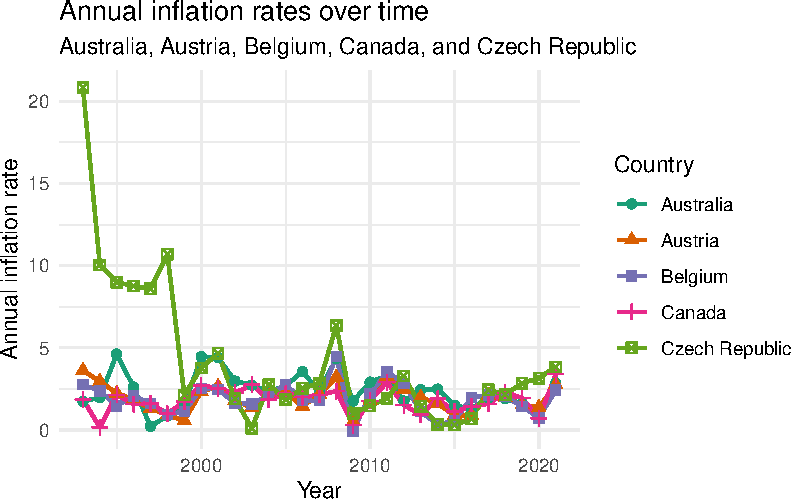
\includegraphics[keepaspectratio]{lab-3_files/figure-pdf/unnamed-chunk-15-1.pdf}}

The plot shows the annual inflation rates for Australia, Austria,
Belgium, Canada, and the Czech Republic between 1993 and 2021. Overall,
the inflation rates for Australia, Austria, Belgium, and Canada appear
relatively stable over time, generally remaining within a moderate range
with only small fluctuations. In contrast, the Czech Republic shows much
larger fluctuations, particularly in the earlier years, where inflation
rates are significantly higher before declining and stabilizing later.
This was surprising to me because I do not have much background
knowledge about the Czech Republic's economy. Without that economic
context, the noticeably greater volatility in its inflation rates
compared to the other four countries stands out as unexpected.

If you haven't yet done so, now is a good time to render, commit, and
push. Make sure that you commit and push all changed documents and your
Git pane is completely empty before proceeding.

\subsection{Part 2}\label{part-2}

\textbf{Inflation in the US}

The OECD defines inflation as follows:

\begin{quote}
Inflation is a rise in the general level of prices of goods and services
that households acquire for the purpose of consumption in an economy
over a period of time.

The main measure of inflation is the annual inflation rate which is the
movement of the Consumer Price Index (CPI) from one month/period to the
same month/period of the previous year expressed as percentage over
time.

Source:
\href{https://www.oecd.org/sdd/prices-ppp/consumerpriceindices-frequentlyaskedquestionsfaqs.htm\#1}{OECD
CPI FAQ}
\end{quote}

CPI is broken down into 12 divisions such as food, housing, health, etc.
Your goal in this part is to create another time series plot of annual
inflation, this time for US only.

The data you will need to create this visualization is spread across two
files:

\begin{itemize}
\tightlist
\item
  \texttt{us-inflation.csv}: Annual inflation rate for the US for 12 CPI
  divisions. Each division is identified by an ID number.
\item
  \texttt{cpi-divisions.csv}: A ``lookup table'' of CPI division ID
  numbers and their descriptions.
\end{itemize}

Let's load both of these files.

\begin{Shaded}
\begin{Highlighting}[]
\NormalTok{us\_inflation }\OtherTok{\textless{}{-}} \FunctionTok{read\_csv}\NormalTok{(}\StringTok{"data/us{-}inflation.csv"}\NormalTok{)}
\NormalTok{cpi\_divisions }\OtherTok{\textless{}{-}} \FunctionTok{read\_csv}\NormalTok{(}\StringTok{"data/cpi{-}divisions.csv"}\NormalTok{)}
\end{Highlighting}
\end{Shaded}

\subsubsection{Question 8}\label{question-8}

a. How many columns and how many rows does the \texttt{us\_inflation}
dataset have? What are the variables in it? Add a brief (1-2 sentences)
narrative summarizing this information.

\begin{Shaded}
\begin{Highlighting}[]
\FunctionTok{glimpse}\NormalTok{(us\_inflation)}
\end{Highlighting}
\end{Shaded}

\begin{verbatim}
Rows: 132
Columns: 4
$ country          <chr> "United States", "United States", "United States", "U~
$ cpi_division_id  <dbl> 1, 1, 1, 1, 1, 1, 1, 1, 1, 1, 1, 2, 2, 2, 2, 2, 2, 2,~
$ year             <dbl> 2011, 2012, 2013, 2014, 2015, 2016, 2017, 2018, 2019,~
$ annual_inflation <dbl> 4.8039240, 2.4539620, 0.9083796, 2.6398010, 1.1677110~
\end{verbatim}

The us\_inflation dataset contains 132 rows and 4 columns. The variables
include country, cpi\_division\_id, year, and annual\_inflation, where
each row represents the inflation rate for the United States for a
specific CPI division and year.

b. How many columns and how many rows does the \texttt{cpi\_divisions}
dataset have? What are the variables in it? Add a brief (1-2 sentences)
narrative summarizing this information.

\begin{Shaded}
\begin{Highlighting}[]
\FunctionTok{glimpse}\NormalTok{(cpi\_divisions)}
\end{Highlighting}
\end{Shaded}

\begin{verbatim}
Rows: 12
Columns: 2
$ id          <dbl> 1, 2, 3, 4, 5, 6, 7, 8, 9, 10, 11, 12
$ description <chr> "Food and non-Alcoholic beverages", "Alcoholic beverages, ~
\end{verbatim}

The cpi\_divisions dataset contains 12 rows and 2 columns. The variables
are id and description, where each row represents a CPI division
category and the description provides the name of the category used in
the Consumer Price Index classification.

c. Create a new dataset by joining the \texttt{us\_inflation} dataset
with the \texttt{cpi\_division\_id} dataset.

\begin{itemize}
\item
  Determine which type of join is the most appropriate one and use that.
\item
  Note that the two datasets don't have a common variable. Review the
  help for the join functions to determine how to use the \texttt{by}
  argument when the names of the variables that the datasets should be
  joined by are different.
\item
  Use a short but informative name for the joined dataset, and do not
  overwrite either of the datasets that go into creating it.
\end{itemize}

Then, find the number of rows and columns of the resulting dataset and
report the names of its columns. Add a brief (1-2 sentences) narrative
summarizing this information.

\begin{Shaded}
\begin{Highlighting}[]
\NormalTok{us\_inflation\_joined }\OtherTok{\textless{}{-}}\NormalTok{ us\_inflation }\SpecialCharTok{\%\textgreater{}\%}
  \FunctionTok{left\_join}\NormalTok{(cpi\_divisions, }\AttributeTok{by =} \FunctionTok{c}\NormalTok{(}\StringTok{"cpi\_division\_id"} \OtherTok{=} \StringTok{"id"}\NormalTok{))}

\FunctionTok{glimpse}\NormalTok{(us\_inflation\_joined)}
\end{Highlighting}
\end{Shaded}

\begin{verbatim}
Rows: 132
Columns: 5
$ country          <chr> "United States", "United States", "United States", "U~
$ cpi_division_id  <dbl> 1, 1, 1, 1, 1, 1, 1, 1, 1, 1, 1, 2, 2, 2, 2, 2, 2, 2,~
$ year             <dbl> 2011, 2012, 2013, 2014, 2015, 2016, 2017, 2018, 2019,~
$ annual_inflation <dbl> 4.8039240, 2.4539620, 0.9083796, 2.6398010, 1.1677110~
$ description      <chr> "Food and non-Alcoholic beverages", "Food and non-Alc~
\end{verbatim}

The joined dataset us\_inflation\_joined contains 132 rows and 5
columns. It includes the variables country, cpi\_division\_id, year,
annual\_inflation, and description, where the description column
provides the CPI division name associated with each inflation
observation.

\subsubsection{Question 9}\label{question-9}

a. Create a vector called \texttt{divisions\_of\_interest} which
contains the descriptions or IDs of CPI divisions you want to visualize.
Your \texttt{divisions\_of\_interest} should consist of no more than
five divisions. If you're using descriptions, make sure that the
spelling of your divisions matches how they appear in the dataset. Then,
in 1-2 sentences, state why you chose these divisions.

\begin{Shaded}
\begin{Highlighting}[]
\NormalTok{divisions\_of\_interest }\OtherTok{\textless{}{-}} \FunctionTok{c}\NormalTok{(}
  \StringTok{"Food and non{-}Alcoholic beverages"}\NormalTok{,}
  \StringTok{"Housing, water, electricity, gas and other fuels"}\NormalTok{,}
  \StringTok{"Transport"}\NormalTok{,}
  \StringTok{"Health"}\NormalTok{,}
  \StringTok{"Education"}
\NormalTok{)}
\end{Highlighting}
\end{Shaded}

These divisions were chosen because I think they represent major
categories of everyday spending, and I want to explore how inflation is
affecting the essentials in a household's expenditure.

\begin{tcolorbox}[enhanced jigsaw, toptitle=1mm, bottomrule=.15mm, colbacktitle=quarto-callout-tip-color!10!white, colframe=quarto-callout-tip-color-frame, leftrule=.75mm, breakable, toprule=.15mm, colback=white, arc=.35mm, coltitle=black, left=2mm, opacitybacktitle=0.6, bottomtitle=1mm, opacityback=0, title=\textcolor{quarto-callout-tip-color}{\faLightbulb}\hspace{0.5em}{Tip}, titlerule=0mm, rightrule=.15mm]

Refer back to the guidance provided in \hyperref[question-6]{Question 6}
if you're not sure how to create this vector.

\end{tcolorbox}

b. In a single pipeline, filter your reshaped dataset to include only
the \texttt{divisions\_of\_interest} from part (a), and save the
resulting data frame with a new name so you (1) can refer to this data
frame later in your analysis and (2) do not overwrite the data frame
you're starting with. Use a short but informative name. Then, in a new
pipeline, find the \texttt{distinct()} divisions in the data frame you
created.

\begin{Shaded}
\begin{Highlighting}[]
\NormalTok{inflation\_divisions }\OtherTok{\textless{}{-}}\NormalTok{ us\_inflation\_joined }\SpecialCharTok{\%\textgreater{}\%}
  \FunctionTok{filter}\NormalTok{(description }\SpecialCharTok{\%in\%}\NormalTok{ divisions\_of\_interest)}

\NormalTok{inflation\_divisions }\SpecialCharTok{\%\textgreater{}\%}
  \FunctionTok{distinct}\NormalTok{(description)}
\end{Highlighting}
\end{Shaded}

\begin{verbatim}
# A tibble: 5 x 1
  description                                     
  <chr>                                           
1 Food and non-Alcoholic beverages                
2 Housing, water, electricity, gas and other fuels
3 Health                                          
4 Transport                                       
5 Education                                       
\end{verbatim}

\subsubsection{Question 10}\label{question-10}

Using your data frame from the previous question, create a plot of
annual inflation vs.~year for these divisions. Then, in a few sentences,
describe the patterns you observe in the plot, particularly focusing on
anything you find surprising or not surprising, based on your knowledge
(or lack thereof) of inflation rates in the US over the last decade.

\begin{itemize}
\tightlist
\item
  Data should be represented with points as well as lines connecting the
  points for each division.
\item
  Each division should be represented by a different color line and
  different color and shape points.
\item
  Axes and legend should be properly labeled.
\item
  The plot should have an appropriate title (and optionally a subtitle).
\item
  Plot should be customized in at least one way -- you could use a
  different than default color scale, or different than default theme,
  or some other customization.
\item
  If your legend has labels that are too long, you can try moving the
  legend to the bottom and stack the labels vertically. \emph{Hint:} The
  \texttt{legend.position} and \texttt{legend.direction} arguments of
  the \texttt{theme()} functions will be useful.
\end{itemize}

\begin{Shaded}
\begin{Highlighting}[]
\FunctionTok{ggplot}\NormalTok{(inflation\_divisions, }
       \FunctionTok{aes}\NormalTok{(}\AttributeTok{x =}\NormalTok{ year, }\AttributeTok{y =}\NormalTok{ annual\_inflation,}
           \AttributeTok{color =}\NormalTok{ description, }\AttributeTok{shape =}\NormalTok{ description, }\AttributeTok{group =}\NormalTok{ description)) }\SpecialCharTok{+}
  \FunctionTok{geom\_line}\NormalTok{(}\AttributeTok{linewidth =} \FloatTok{0.8}\NormalTok{) }\SpecialCharTok{+}
  \FunctionTok{geom\_point}\NormalTok{(}\AttributeTok{size =} \DecValTok{2}\NormalTok{) }\SpecialCharTok{+}
  \FunctionTok{labs}\NormalTok{(}
    \AttributeTok{x =} \StringTok{"Year"}\NormalTok{,}
    \AttributeTok{y =} \StringTok{"Annual inflation rate"}\NormalTok{,}
    \AttributeTok{color =} \StringTok{"CPI division"}\NormalTok{,}
    \AttributeTok{shape =} \StringTok{"CPI division"}\NormalTok{,}
    \AttributeTok{title =} \StringTok{"Annual inflation rates over time by CPI division in the United States"}\NormalTok{,}
    \AttributeTok{subtitle =} \StringTok{"Selected CPI divisions"}
\NormalTok{  ) }\SpecialCharTok{+}
  \FunctionTok{scale\_color\_brewer}\NormalTok{(}\AttributeTok{palette =} \StringTok{"Dark2"}\NormalTok{) }\SpecialCharTok{+}
  \FunctionTok{theme\_minimal}\NormalTok{() }\SpecialCharTok{+}
  \FunctionTok{theme}\NormalTok{(}
    \AttributeTok{legend.position =} \StringTok{"bottom"}\NormalTok{,}
    \AttributeTok{legend.direction =} \StringTok{"vertical"}
\NormalTok{  )}
\end{Highlighting}
\end{Shaded}

\pandocbounded{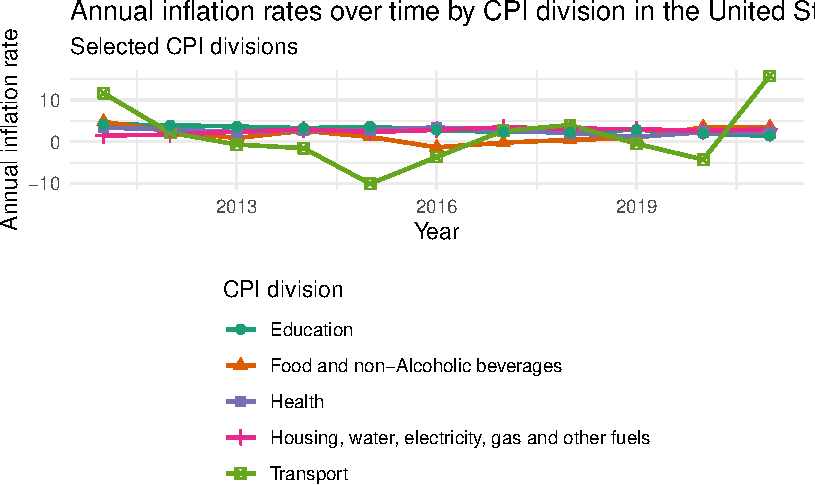
\includegraphics[keepaspectratio]{lab-3_files/figure-pdf/unnamed-chunk-21-1.pdf}}

The plot shows that inflation rates for most of the selected CPI
divisions, including education, health, food and non-alcoholic
beverages, and housing, water, electricity, gas and other fuels, remain
relatively stable over time with only moderate fluctuations. In
contrast, the transport division displays much larger variability, with
noticeable spikes and drops across several years. I found this somewhat
surprising because I initially expected essential categories such as
food and housing to show larger fluctuations compared to transport.
However, I do not have extensive knowledge of the United States economy,
so this pattern may reflect economic factors affecting transportation
costs, such as changes in fuel prices.

If you haven't yet done so since Part 1, now is a good time to render,
commit, and push. Make sure that you commit and push all changed
documents and your Git pane is completely empty before proceeding.

\section{Wrap-up}\label{wrap-up}

\subsection{Submission}\label{submission}

Once you are finished with the lab, you will submit your final PDF
document to Canvas.

\begin{tcolorbox}[enhanced jigsaw, toptitle=1mm, bottomrule=.15mm, colbacktitle=quarto-callout-warning-color!10!white, colframe=quarto-callout-warning-color-frame, leftrule=.75mm, breakable, toprule=.15mm, colback=white, arc=.35mm, coltitle=black, left=2mm, opacitybacktitle=0.6, bottomtitle=1mm, opacityback=0, title=\textcolor{quarto-callout-warning-color}{\faExclamationTriangle}\hspace{0.5em}{Warning}, titlerule=0mm, rightrule=.15mm]

Before you wrap up the assignment, make sure all of your documents are
updated on your GitHub repo. We will be checking these to make sure you
have been practicing how to commit and push changes.

You must turn in a PDF file to the Canvas page by the submission
deadline to be considered ``on time''.

\end{tcolorbox}

To submit your assignment:

\begin{itemize}
\tightlist
\item
  Go to \url{http://www.Canvas.com} and click \emph{Log in} in the top
  right corner.
\item
  Click \emph{School Credentials} \(\rightarrow\) \emph{Duke NetID} and
  log in using your NetID credentials.
\item
  Click on your \emph{REN R 213} course.
\item
  Click on the assignment, and you'll be prompted to submit it.
\item
  Mark all the pages associated with question. All the pages of your lab
  should be associated with at least one question (i.e., should be
  ``checked'').
\end{itemize}

\begin{tcolorbox}[enhanced jigsaw, toptitle=1mm, bottomrule=.15mm, colbacktitle=quarto-callout-important-color!10!white, colframe=quarto-callout-important-color-frame, leftrule=.75mm, breakable, toprule=.15mm, colback=white, arc=.35mm, coltitle=black, left=2mm, opacitybacktitle=0.6, bottomtitle=1mm, opacityback=0, title=\textcolor{quarto-callout-important-color}{\faExclamation}\hspace{0.5em}{Checklist}, titlerule=0mm, rightrule=.15mm]

Make sure you have:

\begin{itemize}
\tightlist
\item
  attempted all questions
\item
  rendered your Quarto document
\item
  committed and pushed everything to your GitHub repository such that
  the Git pane in RStudio is empty
\item
  uploaded your PDF to Canvas
\item
  selected pages associated with each question on Canvas
\end{itemize}

\end{tcolorbox}

\subsection{Grading}\label{grading}

The lab is graded out of a total of 36 points.

You can earn up to 4 points on each question:

\begin{itemize}
\item
  4: Response shows excellent understanding and addresses all or almost
  all of the rubric items.
\item
  3: Response shows good understanding and addresses most of the rubric
  items.
\item
  2: Response shows understanding and addresses a majority of the rubric
  items.
\item
  1: Response shows effort and misses many of the rubric items.
\item
  0: Response does not show sufficient effort or understanding and/or is
  largely incomplete.
\end{itemize}




\end{document}
